\documentclass[11pt,letterpaper]{article}
\usepackage[utf8]{inputenc} %Codificacion del texto (ISO Latin1 encoding)

\usepackage{fancyhdr} %Permite acomodar a tu gusto la parte de arriba y
% abajo del documento
\usepackage[spanish]{babel} %Permite definir el idioma del dcumento
\usepackage{graphicx} %Permite exportar imagenes en formato eps
\usepackage{url} %Tipo de fuente para correos y paginas
\usepackage{pgf}
\usepackage{fleqn}
\usepackage{amssymb}
\usepackage{fancyvrb}
\usepackage{sectsty}
\usepackage{makeidx}
\usepackage{colortbl} %Permite colocar colores a las tablas
\usepackage{booktabs}
%%%%%%%%%%
%Margenes%
%%%%%%%%%%
\parskip 1mm %Espacio entre parrafos

\setlength{\topmargin}{0pt}

\oddsidemargin	0.5cm  % Ancho Letter 21,59cm
\evensidemargin 0.5cm  % Alto  Letter 27,81cm
\textwidth	15.5cm
\textheight	21.0cm
\headsep	4 mm
\parindent	0.5cm
%%%%%%%%%%%%%%%%%%%%%%
%Estilo del documento%
%%%%%%%%%%%%%%%%%%%%%%
\pagestyle{fancyplain}

%%%%%%%%%%%%%%%%%%%%%%%%%%%%%%%%%%%%%%%%%%%
%Fancyheadings. Top y Bottom del documento%
%%%%%%%%%%%%%%%%%%%%%%%%%%%%%%%%%%%%%%%%%%%
% Recuerde que en este documento la portada del documento no posee
% numeracion, pero de igual manera llamaremos a esa primera pagina la numero
% 1, y la que viene la dos. Esto es para tener una idea de las que
% llamaremos pares e impares
\lhead{Fundamentos de Ingeniería de Software} %Parte superior izquierda
\rhead{\bf \it Tarea 2} %Parte superior derecha
\lfoot{\it Octubre 2008} %Parte inferior izquierda. \thepage indica
% el numero de pagina
\cfoot{} %Parte inferior central
\rfoot{\bf \thepage} %Parte inferior derecha
\renewcommand{\footrulewidth}{0.4pt} %Linea de separacion inferior

% Challa

\newtheorem{theorem}{Theorem}
\newtheorem{acknowledgement}[theorem]{Acknowledgement}
\newtheorem{algorithm}[theorem]{Algorithm}
\newtheorem{axiom}[theorem]{Axiom}
\newtheorem{case}[theorem]{Case}
\newtheorem{claim}[theorem]{Claim}
\newtheorem{conclusion}[theorem]{Conclusion}
\newtheorem{condition}[theorem]{Condition}
\newtheorem{conjecture}[theorem]{Conjecture}
\newtheorem{corollary}[theorem]{Corollary}
\newtheorem{criterion}[theorem]{Criterion}
\newtheorem{definition}[theorem]{Definition}
\newtheorem{example}[theorem]{Example}
\newtheorem{exercise}[theorem]{Exercise}
\newtheorem{lemma}[theorem]{Lemma}
\newtheorem{notation}[theorem]{Notation}
\newtheorem{problem}[theorem]{Problem}
\newtheorem{proposition}[theorem]{Proposition}
\newtheorem{remark}[theorem]{Remark}
\newtheorem{solution}[theorem]{Solution}
\newtheorem{summary}[theorem]{Summary}
\newenvironment{proof}[1][Proof]{\noindent\textbf{#1.} }{\ \rule{0.5em}{0.5em}}

\newcommand{\primaria}[1]{
	\textbf{\underline{#1}}
}

\newcommand{\foranea}[1]{
	\textbf{\textsl{#1}}
}

\newcommand{\primyfor}[1]{
	\underline{\foranea{#1}}
}

\makeatletter
\newcommand\subsubsubsection{\@startsection {paragraph}{1}{\z@}%
                                   {-3.5ex \@plus -1ex \@minus -.2ex}%
                                   {1.5ex \@plus.2ex}%
                                   {\normalfont\bfseries}}
\newcommand\subsubsubsubsection{\@startsection {subparagraph}{1}{\z@}%
                                   {-3.5ex \@plus -1ex \@minus -.2ex}%
                                   {1.5ex \@plus.2ex}%
                                   {\normalfont\bfseries}}


\makeatother

%\makeindex
%%%%%%%%%%%%%%%%%%%%%%%%%%%%%%%%%%%%%%%%%%%%%%%%%%%%%%%%%%%%%%%%%%%
%%%%%%%%%%%%%%%%%%%% Aqui empieza el documento %%%%%%%%%%%%%%%%%%%%
%%%%%%%%%%%%%%%%%%%%%%%%%%%%%%%%%%%%%%%%%%%%%%%%%%%%%%%%%%%%%%%%%%%

\begin{document}

%%%%%%%%%%%%%%%%%%%%%%%%%%
%Definicion de la portada%
%%%%%%%%%%%%%%%%%%%%%%%%%%
\begin{titlepage}
    \begin{center}
	\begin{tabular}{ccc}
	    %\epsfig{file=escudo-utfsm.eps, height=1.6cm}
	      
\includegraphics[height=1.6cm]{images/logoUTFSM}
	    & %Escudo de la Universidad Santa Maria
	    \hspace{0.2cm}
	    \begin{tabular}{c}
		Universidad Técnica Federico Santa María \\ \hline
		\hspace{8.0cm}
		\vspace{1.2cm}
	    \end{tabular}
	    \hspace{0.2cm}
	    &
	   % \epsfig{file=logo_DI.eps, height=1.6cm} %Logo del DI
            
\includegraphics[height=1.6cm]{images/logoDI}
	\end{tabular}

	\vspace{2.5cm}
	%Titulo del Documento
	    \begin{tabular}{c}
		\Huge{\textbf{Tarea 2}}\\\\\\\\\\\\\\
		\LARGE{\textbf{``Sistema de Gesti\'on de Clientes VIP''}}\\\\
		\LARGE{\sc{Fundamentos de Ingenier\'ia}}\\
		\LARGE{\sc{de Software}}
	    \end{tabular}

	\vspace{2.5cm}
%	\begin{tabular}{c}
	\begin{center}
%	     \pgfimage[height=1.8cm]{images/now}
	%    \Huge{\emph{Now!}}
%	\end{tabular}
	\end{center}
	
        \vspace{1.5cm}

	%Nombre del (o los) autor(es)
	\begin{tabular}{lr}
            \begin{tabular}{c}
	        \large{Rodrigo Fern\'andez - 2673002-3}\\
		\large{\url{rfernand@inf.utfsm.cl}}
	    \end{tabular}
	&
	   \begin{tabular}{c}
         	\large{Cristi\'an Maureira - 2673030-9}\\ 
		\large{\url{cmaureir@inf.utfsm.cl}}
	   \end{tabular}
	\end{tabular}
        \vspace{3.5cm}\\
	%Fecha
		\large{\sc{Valpara\'iso, Octubre 2008.}}
    \end{center}
\end{titlepage}


\section{Modelamiento Estatico}
\label{sec:modelamiento_estatico}
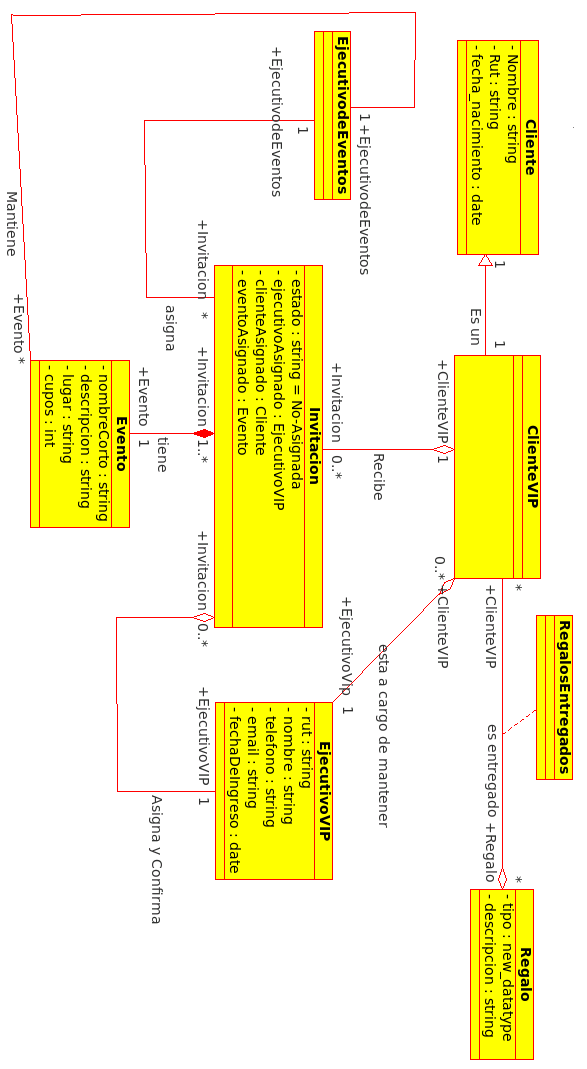
\includegraphics[height=19.5cm,width=11.5cm]{images/modeloEstatico}


\section{Modelamiento Dinamico}
\subsection{Diagrama de Casos de Uso}
\label{sec:diagramacasosdesuso}
\includegraphics[height=19.5cm,width=11.5cm]{images/casoDeUso_2}

\subsection{Casos de Uso de Alto Nivel}
\label{sec:casosdeuso_altonivel}
\subsubsection{Clientes y Ejecutivos VIP}

\begin{itemize}
	\item Mantener Clientes VIP\\
		\begin{tabular}[5 cm]{|c|p{11cm}|}\hline
			Caso de Uso: & Mantener Clientes VIP\\\hline
			Actores: & Administrador de Sistema\\\hline
			Tipo: & Esencial, Primario\\\hline
			Descripción: & El Sistema permite Crear, Obtener, Actualizar y Borrar (CRUD) Clientes VIP\\\hline
		\end{tabular}

	\item Editar Clientes VIP\\
		\begin{tabular}[5 cm]{|c|p{11cm}|}\hline
			Caso de Uso: & Editar Clientes VIP\\\hline
			Actores: & Administrador del Sistema\\\hline
			Tipo: & Esencial, Secundario\\\hline
			Descripción: & El Sistema permite la edición de los datos de los Clientes VIP\\\hline
		\end{tabular}

	\item Obtener Información del Cliente\\
		\begin{tabular}{|c|p{11cm}|}\hline
			Caso de Uso: & Obtener Información del Cliente\\\hline
			Actores: & SCR, Administrador del Sistema\\\hline
			Tipo: & Esencial, Primario\\\hline
			Descripción: &El Sistema permite obtener toda la información del Clienete desde el SCR\\\hline
		\end{tabular}

	\item Mantener Ejecutivos Clientes VIP\\
		\begin{tabular}{|c|p{11cm}|}\hline
			Caso de Uso: & Mantener Ejecutivos Clientes VIP\\\hline
			Actores: &Administrador del Sistema\\\hline
			Tipo: & Esencial, Primario\\\hline
			Descripción: & Crear, Obtener, Actualizar y Borrar (CRUD) Ejecutivos de Clientes VIP\\\hline
		\end{tabular}

	\item Editar Ejecutivo Clientes VIP\\
		\begin{tabular}{|c|p{11cm}|}\hline
			Caso de Uso: & Editar Ejecutivo Clientes VIP\\\hline
       			Actores: &Administrador del Sistema\\\hline
			Tipo: & Esencial, Secundario\\\hline
			Descripción: &El Sistema permite la edición de los datos de los Ejecutivos de Clientes VIP\\\hline
		\end{tabular}
\end{itemize}


\subsubsection{Eventos}

\begin{itemize}
	\item Mantener Eventos\\
		\begin{tabular}{|c|p{11cm}|}\hline
			Caso de Uso: & Mantener Eventos\\\hline
			Actores: & Administrador de Eventos\\\hline
			Tipo: & Esencial, Primario\\\hline
			Descripción: & Crear, Obtener, Actualizar y Borrar (CRUD) Eventos\\\hline
		\end{tabular}

	\item Editar Evento\\
		\begin{tabular}{|c|p{11cm}|}\hline
			Caso de Uso: & Editar Evento\\\hline
			Actores: & Administrador de Eventos\\\hline
			Tipo: & Esencial, Secundario\\\hline
			Descripción: &El Sistema permite la edición de los datos de los Eventos\\\hline
		\end{tabular}

	\item Administrar Invitaciones de Evento\\
		\begin{tabular}{|c|p{11cm}|}\hline
			Caso de Uso: & Administrar Invitaciones de Evento\\\hline
			Actores: &Administrador de Eventos\\\hline
			Tipo: & Esencial, Primario\\\hline
			Descripción: &El Administrador de Eventos debe poder permitir administrar las invitaciones de cada evento para que los Ejecutivos puedan enviar invitaciones a los Clientes VIP\\\hline
		\end{tabular}

	\item Administrar Invitaciones\\
		\begin{tabular}{|c|p{11cm}|}\hline
			Caso de Uso: & Administrar Invitaciones\\\hline
			Actores: & Ejecutivo VIP\\\hline
			Tipo: & Esencial, Primario\\\hline
			Descripción: &El Ejecutivo VIP debe poder administrar las invitaciones, llevando un registro\\\hline
		\end{tabular}

	\item Asignar Invitaciones a Cliente VIP\\
		\begin{tabular}{|c|p{11cm}|}\hline
			Caso de Uso: & Asignar Invitaciones a Clientes VIP\\\hline
			Actores: &Ejecutivo VIP\\\hline
			Tipo: & Esencial, Secundario\\\hline
			Descripción: &El Ejecutivo VIP debe poder asignar una invitación a un Cliente VIP\\\hline
		\end{tabular}

\end{itemize}
\subsubsection{Regalos}

\begin{itemize}
	\item Consultar Próximos Cumpleaños\\
		\begin{tabular}{|c|p{11cm}|}\hline
			Caso de Uso: & Consultar Próximos Cumpleaños\\\hline
			Actores: &Ejecutivo VIP\\\hline
			Tipo: & Esencial, Primario\\\hline
			Descripción: &El Ejecutivo VIP debe poder consultar sobre los próximos cumpleaños para poder realizar su trabajo\\\hline
		\end{tabular}

	\item Mantener Regalos\\
		\begin{tabular}{|c|p{11cm}|}\hline
			Caso de Uso: & Mantener Regalos\\\hline
			Actores: & Administrador del Sistema\\\hline
			Tipo: & Esencial, Primario\\\hline
			Descripción: & Crear, Obtener, Actualizar y Borrar (CRUD) Regalos\\\hline
		\end{tabular}

	\item Editar Regalo\\
		\begin{tabular}{|c|p{11cm}|}\hline
			Caso de Uso: & Editar Regalo \\\hline
			Actores: & Administrador del Sistema\\\hline
			Tipo: & Esencial, Secundario\\\hline
			Descripción: &El Sistema permite la edición de los datos de los Regalos\\\hline
		\end{tabular}

	\item Asignar Regalo\\
		\begin{tabular}{|c|p{11cm}|}\hline
			Caso de Uso: & Asignar Regalo\\\hline
			Actores: &Ejecutivo VIP\\\hline
			Tipo: & Esencial, Secundario\\\hline
			Descripción: &El Ejecutivo VIP permite la asignación de un regalo a un Cliente VIP\\\hline
		\end{tabular}

	\item Ver Historial de Regalos de Cliente\\
		\begin{tabular}{|c|p{11cm}|}\hline
			Caso de Uso: & Ver Historial de Regalos de Clientes\\\hline
			Actores: &Ejecutivo VIP\\\hline
			Tipo: & Esencial, Secundario\\\hline
			Descripción: &El Ejecutivo debe poder ver el historial de regalos de Clientes VIP para que no se repita\\\hline
		\end{tabular}
\end{itemize}


\subsection{Casos de Uso Expandidos}
\label{sec:casosdeuso_expandido_regalos}
\subsubsection{Mantener Regalo}
\begin{itemize}
	\item Caso de Uso Expandido\\
		\begin{tabular}{|c|p{9.5cm}|}\hline
			Caso de Uso: & Mantener Regalo  \\\hline
			Actores: & Administrador del Sistema \\\hline
			Propósito: & Agregar, Modificar y Eliminar Regalos \\\hline
			Resumen: & El Administrador del Sistema es capaz realizar las mantenciones de la base de datos de los regalos agregando, modificando o eliminandolos.\\\hline
			Tipo: & Esencial, Primario \\\hline
			Descripción: & El administrador elige el tipo de mantencion que quiere realizar y dependiendo del caso, seleccionar de una lista los regalos a modificar o eliminar, pudiendo ver los detalles de cada uno antes de confirmar la operaci\'on  \\\hline
			Referencias Cruzadas: & Modificar Regalo \\\hline
		\end{tabular}

	\item Curso Normal de Eventos: Ingresar Regalo\\
		\begin{tabular}{|p{6.6cm}|p{6.6cm}|}\hline
			\emph{Acción del Actor} & \emph{Respuesta del Sistema}\\\hline
			1. El Administrador del Sistema entra a Mantener Regalos&\\\hline
			&2. El Sistema despliega las 4 opciones permitidas(agregar, modificar, eliminar, volver)\\\hline
			3. El Administrador del Sistema elige agregar Regalo&\\\hline
			&4. El Sistema consulta los atributos del regalo\\\hline
			5. El Administrador del Sistema rellena los atributos requeridos&\\\hline
			&6. El Sistema verifica la integridad de los datos\\\hline
			7. El Administrador confirma el ingreso&\\\hline
			&8. El Sistema ingresa el nuevo regalo a la base de datos y avisa de que la agregaci\'on fue realizada con \'exito\\\hline
			&9. El Sistema regresa al punto 2. \\\hline
		\end{tabular}

	\item Curso Alternativo de Eventos  \\
		\begin{tabular}{|p{6.6cm}|p{6.6cm}|}\hline
			\emph{Acción del Actor} & \emph{Respuesta del Sistema}\\\hline
			&8. El Sistema indica que ya existe ese regalo y regresa al punto 2 \\\hline
			&\\\hline
			3. El Administrador del Sistema elige eliminar Regalo& \\\hline
			&4. El Sistema despliega los 10 ultimos regalos agregados y una casilla para buscar regalos\\\hline
			5. El Administrador selecciona un Regalo de la lista&\\\hline
			&6. El Sistema le muestra los atributos del Regalo y pregunta si realmente desea elminar este regalo\\\hline
			7. El Administrador confirma la eliminaci\'on&\\\hline
			&8. El Sistema elimina de la base de datos al regalo y avisa de que la eliminaci\'on fue realizada con \'exito. Regreso al punto 2\\\hline
			&\\\hline
			8. El Regalo fue modificado o eliminado en el proceso por otro Administrador & 9. El sistema notifica que la operacion no pudo ser realizada y tira un error de eliminaci\'on. Regreso al punto 2  \\\hline
		\end{tabular}
\end{itemize}

\subsubsection{Editar Regalo}
\begin{itemize}
	\item Caso de Uso Expandido\\
		\begin{tabular}{|c|p{9.5cm}|}\hline
			Caso de Uso: & Editar Regalo\\\hline
			Actores: & Administrador del Sistema\\\hline
			Propósito: & Editar los atributos de cierto regalo\\\hline
			Resumen: & El Administrador del Sistema es capaz de modificar de forma integra los atributos de un Regalo\\\hline
			Tipo: & Esencial, Secundario \\\hline
			Descripción: & El administrador elige el regalo a modificar, para luego elegir uno de sus atributos y modificar uno de ellos. El Sistema verifica los atributos para mantener la integridad de los datos\\\hline
			Referencias Cruzadas: & Mantener Regalo \\\hline
		\end{tabular}

	\item Curso Normal de Eventos\\
		\begin{tabular}{|p{6.6cm}|p{6.6cm}|}\hline
			\emph{Acción del Actor} & \emph{Respuesta del Sistema}\\\hline
			& 1. El Sistema despliega un menu para buscar un regalo por alguno de sus atributos\\\hline
			2. El Administrador selecciona un atributo, ingresa alguna palabra clave para realizar la busqueda, y presiona en buscar&\\\hline
			& 3. El Sistema despliega una lista de los regalos que coinciden con la palabra clave (manteniendo el menu de busqueda en la pantalla)\\\hline
			4. El Administrador elige uno de los regalos desplegados&\\\hline
			& 5. El Sistema despliega el detalle de Regalo con sus atributos en casillas modificables\\\hline
			6. El Administrador modifica algun atributo y presiona modificar&\\\hline
			& 7. El Sistema verifica que todos los campos esten bien ingresados y que no existan duplicados del mismo regalo\\\hline
			& 8. El Sistema realiza la modificaci\'on en la base de datos, y muestra por pantalla que la modificaci\'on fue realizada con exito \\\hline
			& 9. El Sistema se regresa al Curso Normal de Eventos de Mantener Regalo, paso 2.\\\hline
		\end{tabular}

	\item Curso Alternativo de Eventos\\
		\begin{tabular}{|p{6.6cm}|p{6.6cm}|}\hline
			\emph{Acción del Actor} & \emph{Respuesta del Sistema}\\\hline
			4. No se encontraron coincidencias & 5. El Sistema avisa de que no existe ningun Regalo que coincida con alguno de esos atributos y vuelve al punto 1. \\\hline
			8. El sistema detecta que el Regalo ya fue modificado o eliminado por otro administrador& 9. El Sistema tira un error de edici\'on y notifica que la modificaci\'on no pudo ser realizada porque el Regalo ya no existe.\\\hline
			& 10. El Sistema se regresa al Curso Normal de Eventos de Mantener Regalo, paso 2.\\\hline
		\end{tabular}

\end{itemize}


\label{sec:casosdeuso_expandido}
%\subsubsection{Mantener Regalo}
%\begin{itemize}
%	\item Caso de Uso Expandido\\
%		\begin{tabular}{|c|p{9.5cm}|}\hline
%			Caso de Uso: & \\\hline
%			Actores: & \\\hline
%			Propósito: & \\\hline
%			Resumen: & \\\hline
%			Tipo: & \\\hline
%			Descripción: & \\\hline
%			Referencias Cruzadas: & \\\hline
%		\end{tabular}
%
%	\item Curso Normal de Eventos\\
%		\begin{tabular}{|p{6.6cm}|p{6.6cm}|}\hline
%			\emph{Acción del Actor} & \emph{Respuesta del Sistema}\\\hline
%			&\\\hline
%			&\\\hline
%			&\\\hline
%		\end{tabular}
%
%	\item Curso Alternativo de Eventos\\
%		\begin{tabular}{|p{6.6cm}|p{6.6cm}|}\hline
%			\emph{Acción del Actor} & \emph{Respuesta del Sistema}\\\hline
%			&\\\hline
%			&\\\hline
%			&\\\hline
%		\end{tabular}
%
%\end{itemize}
%
%\subsubsection{Editar Regalo}
%\begin{itemize}
%	\item Caso de Uso Expandido\\
%		\begin{tabular}{|c|p{9.5cm}|}\hline
%			Caso de Uso: & \\\hline
%			Actores: & \\\hline
%			Propósito: & \\\hline
%			Resumen: & \\\hline
%			Tipo: & \\\hline
%			Descripción: & \\\hline
%			Referencias Cruzadas: & \\\hline
%		\end{tabular}
%
%	\item Curso Normal de Eventos\\
%		\begin{tabular}{|p{6.6cm}|p{6.6cm}|}\hline
%			\emph{Acción del Actor} & \emph{Respuesta del Sistema}\\\hline
%			&\\\hline
%			&\\\hline
%			&\\\hline
%		\end{tabular}
%
%	\item Curso Alternativo de Eventos\\
%		\begin{tabular}{|p{6.6cm}|p{6.6cm}|}\hline
%			\emph{Acción del Actor} & \emph{Respuesta del Sistema}\\\hline
%			&\\\hline
%			&\\\hline
%			&\\\hline
%		\end{tabular}
%
%\end{itemize}

\subsubsection{Asignar Invitaciones a Cliente VIP}
\begin{itemize}
	\item Caso de Uso Expandido\\
		\begin{tabular}{|c|p{9.5cm}|}\hline
			Caso de Uso: & Asignar Invitaciones a Cliente VIP\\\hline
			Actores: & Ejecutivo del Cliente VIP\\\hline
			Propósito: & Poder asignar invitaciones de un evento determinado a algún Cliente VIP\\\hline
			Resumen: & El Ejecutivo del Cliente VIP, posee el privilegio de poder asignar una cantidad de entradas a algún Cliente VIP para que éste pueda asistir a dicho evento\\\hline
			Tipo: & Esencial, Secundario\\\hline
			Descripción: &El Ejecutivo del Cliente VIP debe poder asignar una invitación a un Cliente VIP \\\hline
			Referencias Cruzadas: & Administrar Invitaciones\\\hline
		\end{tabular}

	\item Curso Normal de Eventos\\
		\begin{tabular}{|p{6.6cm}|p{6.6cm}|}\hline
			\emph{Acción del Actor} & \emph{Respuesta del Sistema}\\\hline
			1.Administrar Invitaciones&\\\hline
			&2.Se despliega un menu con las opciones para poder administrar las invitaciones\\\hline
			3.Selecciona opción de Asignar Invitaciones a CVIP&\\\hline
			&4.Se despliega un listado con los eventos y clientes disponibles\\\hline
			5.Selecciona un evento y un cliente, con una cierta cantidad de invitaciones&\\\hline
			6.Guarda los cambios&\\\hline
			&7.Vuelve al menu principal\\\hline
			8.Sale del sistema de administración&\\\hline
		\end{tabular}

	\item Curso Alternativo de Eventos\\
		\begin{tabular}{|p{6.6cm}|p{6.6cm}|}\hline
			\emph{Acción del Actor} & \emph{Respuesta del Sistema}\\\hline
			5.No hay eventos disponibles&Se envia un mensaje de error diciendo que no hay eventos disponibles\\\hline
			5.Se envian mas invitaciones de las cuales el evento tiene disponible&Se envia un mensaje de error diciendo que la cantidad de invitaciones no es válida\\\hline
			5.Se cancela un evento justo en el momento de la elección&Se envia un mensaje de error diciendo que el evento ya no esta mas tiempo disponible\\\hline
			5.Se agotan las invitaciones justo en el momento que se esta haciendo la asignación&Se envia un error diciendo que ya no hay invitaciones disponibles para el evento\\\hline
		\end{tabular}

\end{itemize}


\section{Supuestos}
\label{sec:supuestos}
\begin{itemize}
	\item Consideramos que seria bueno que el Administrador de Eventos sea identificable para poder reconocer a posterioridad que administrador de Eventos realizo los mejores eventos, o cometio errores al realizar algo.
	\item Se considero que el curso normal de los eventos, pueden haber diferentes Adminsitradores del Sistema trabajando paralelamente, por lo que habia que validar los datos para evitar inconsistencias en la base de datos.
	\item Se adapt\'o el diagrama de casos de uso segun la pauta dada en la tarea.
	\item Se considero que seg\'un el texto, el que manten\'ia los eventos era el Administrador de Eventos y no el Administrador del Sistema.
\end{itemize}


\section{Descripci\'on herramienta utilizada: Umbrello}
\label{sec:umbrello}
\begin{center}
	
\includegraphics[height=1.5cm]{images/umbrello}\\
\end{center}
\textbf{Umbrello} es una herramienta libre para crear y editar diagramas UML, que ayuda en el proceso del desarrollo de software. Fue desarrollada por Paul Hensgen, y está diseñado principalmente para KDE, aunque funciona en otros entornos de escritorio.\\

Umbrello maneja gran parte de los diagramas estándar UML pudiendo crearlos, además de manualmente, importándolos a partir de código en C++, Java, Python, IDL, Pascal/Delphi, Ada, o también Perl (haciendo uso de una aplicación externa). Así mismo, permite crear un diagrama y generar el código automáticamente en los lenguajes antes citados, entre otros. El formato de fichero que utiliza está basado en XMI.\\

También permite la distribución de los modelos exportándolos en los formatos DocBook y XHTML, lo que facilita los proyectos colaborativos donde los desarrolladores no tienen acceso directo a Umbrello o donde los modelos van a ser publicados vía web.Umbrello se distribuye en el módulo kdesdk de KDE.\\

\textbf{Web:} http://uml.sourceforge.net/


\end{document}
